% generated by make_split.py from the full manuscript (sections_full_20261117); edit here from now on


\section{Chord Inversion in Unconstrained Parameterizations}
\label{sec:ablation_study}
In conventional aircraft conceptual design, wing geometry is naturally regularized by discrete physical sub-assemblies: a discrete fuselage establishes the wing root, and continuous structural spars enforce tapering chords toward the wingtips~\cite{raymer2018aircraft}. In tailless Blended Wing Body configurations, however, the aerodynamic surface represents a continuous spatial progression where the center-body, transition blend station, and outer wing panels are parameterized simultaneously~\cite{samareh2001survey}.

When optimization parameterizations treat station chords as independent variables without relational constraints, the optimizer is permitted to explore configurations where the blend station chord exceeds the root chord ($c_{b} > c_{r}$). In potential-flow solvers, expanding the outboard chord artificially increases circulation without triggering flow detachment, because Laplace's equation does not model adverse pressure gradients or boundary layer separation~\cite{katz2001low}. Such planforms have a larger wetted area and a lower aspect ratio (Table~\ref{tab:ablation}), and the question examined here is whether chord inversion carries an aerodynamic cost beyond that.

\begin{figure}[htbp]
\centering
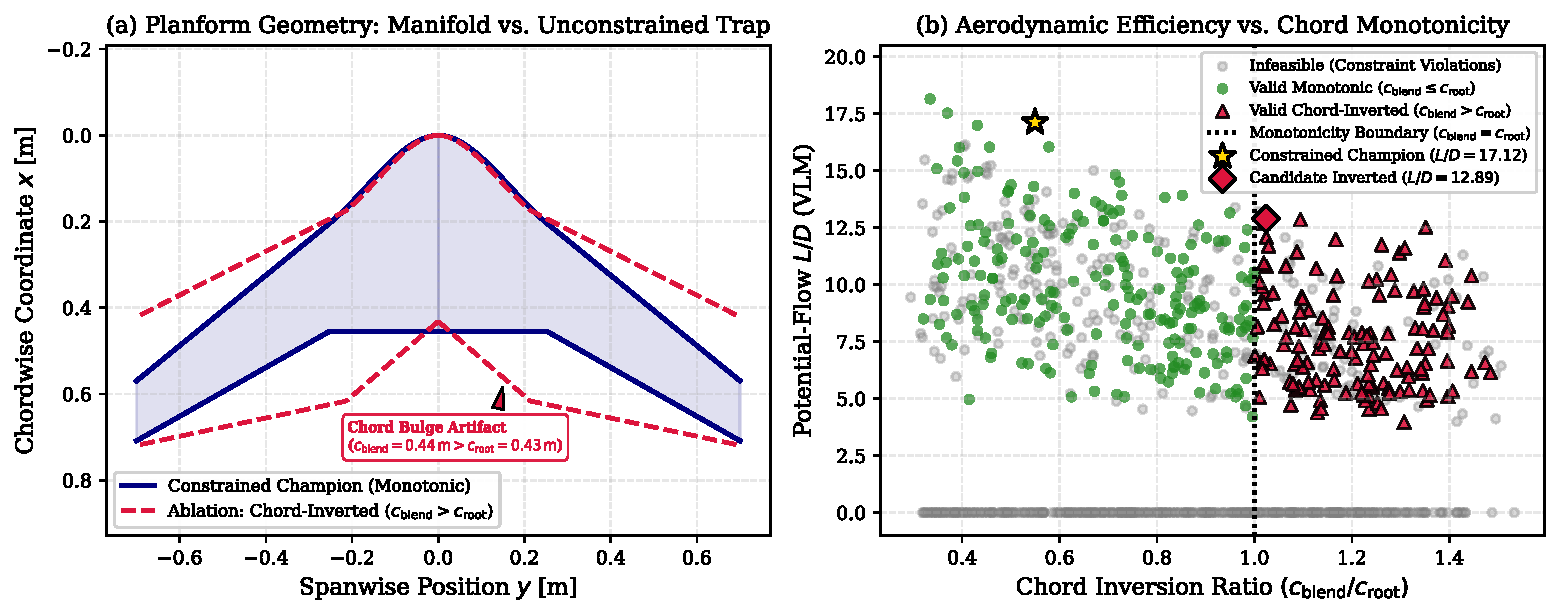
\includegraphics[width=\linewidth]{figures/figure1_ablation_chord_inversion.pdf}
\caption{Quantitative ablation study evaluating the aerodynamic impact of chord monotonicity across $1{,}000$ Latin Hypercube samples. (a) Planform geometry comparison between the clamped original-campaign champion ($L/D = 17.12$, solid navy) and a representative chord-inverted configuration ($c_{b} > c_{r}$, $L/D = 12.89$, dashed crimson). (b) Aerodynamic efficiency ($L/D$) versus chord inversion ratio ($c_{b}/c_{r}$); chord-inverted designs (crimson triangles) exhibit 29\% lower maximum aerodynamic efficiency in the unconstrained sample, an effect confounded by reference area ($S_{\mathrm{ref}} = 0.69$ vs $0.46\,\mathrm{m}^2$); when matched by reference area, efficiency differences narrow to statistical insignificance ($p=0.49$).}
\label{fig:ablation_study}
\end{figure}

To quantify the prevalence and aerodynamic penalty of this artifact, a 1,000-sample Latin Hypercube Sampling (LHS) campaign was conducted with uncoupled bounds on the blend chord ($c_{b} \in [0.15, 0.65]\,\mathrm{m}$). As documented in Table~\ref{tab:ablation} and Fig.~\ref{fig:ablation_study}, $35.5\%$ of generated configurations suffered chord inversion ($355$ out of $1{,}000$ designs). The maximum lift-to-drag ratio discovered among chord-inverted configurations was $(L/D)_{\max} = 12.89$, compared to $(L/D)_{\max} = 18.15$ for monotonic planforms, a 29\% lower maximum aerodynamic efficiency. Across the full distributions of valid designs the mean efficiency is also lower for chord-inverted configurations ($\NAbLDinv$ versus $\NAbLDmono$, $p < 0.001$, Mann--Whitney $U$ test); the $p$-value refers to this comparison of distributions and not to the two maxima.

\begin{table}[htbp]
\centering\small
\caption{Aerodynamic and geometric comparison from the 1,000-sample unconstrained chord ablation experiment.}
\label{tab:ablation}
\begin{tabular}{@{}lrr@{}}
\toprule
 & Chord-inverted & Monotone \\
\midrule
Designs (valid) & 355 (137) & 645 (212) \\
Mean $S_\mathrm{ref}$ (m$^2$) & 0.69 & 0.46 \\
Mean aspect ratio & 3.27 & 5.17 \\
Mean $L/D$, all valid & 7.65 & 9.82 \\
Mean $L/D$, $S_\mathrm{ref}\in[0.53,0.67]$ (n=40, 65) & 8.13 & 8.41 \\
\bottomrule
\end{tabular}

\end{table}

This 29\% gap in maximum efficiency is substantially confounded by planform area. In the unconstrained LHS sample, chord-inverted designs had significantly larger average reference areas ($S_{\mathrm{ref}} = 0.69\,\mathrm{m}^2$ versus $0.46\,\mathrm{m}^2$) and lower aspect ratios ($3.27$ versus $5.17$). When candidates are matched across a common reference area window ($S_{\mathrm{ref}} \in [0.53, 0.67]\,\mathrm{m}^2$, comprising 40 inverted and 65 monotonic designs), the mean efficiency difference becomes statistically indistinguishable: $L/D = 8.13$ for inverted configurations versus $8.41$ for monotonic configurations ($p = 0.49$, Mann--Whitney $U$ test). In an ordinary least-squares regression of $L/D$ on an inversion indicator together with reference area, cruise speed, battery mass and static margin, the coefficient of the indicator is $+0.63 \pm 0.18$ (standard error), that is, slightly in favor of the inverted designs once the covariates are held fixed. The sample therefore gives no evidence that chord inversion by itself lowers the efficiency computed by this pipeline; the raw gap reflects the larger area and lower aspect ratio of the inverted designs. The comparison is observational (the two groups were not designed to differ in one factor only), so it does not show that inversion is harmless either.



\section{Controlled Loft and Bound Experiments: Tables}
\label{sec:supp_loft_tables}
Tables~\ref{tab:loft} and~\ref{tab:bound} belong to Sections~\ref{sec:loft} and~\ref{sec:bound_sensitivity} of the main text, and Table~\ref{tab:mass} to Section~\ref{sec:dynamic_balance}.

\begin{table}[htbp]
\centering\small
\caption{Controlled searches testing the chord clamp and the sensitivity to the bounds (ten seeds each, 287 evaluations, no pool).}
\label{tab:loft}
\resizebox{\linewidth}{!}{%
\begin{tabular}{@{}lrrrrr@{}}
\toprule
Search & Seeds & Best per seed (km) & Mean (km) & Valid (\%) & Inverted / clamp-active samples (\%) \\
\midrule
Clamp (widened $c_b\in[0.15,0.65]$) & 10 & 388, 353, 403, 392, 375, 350, 400, 262, 355, 269 & 354.7 & 55 & 7 \\
No clamp (same bounds) & 10 & 322, 314, 386, 417, 396, 379, 346, 301, 366, 273 & 350.0 & 47 & 7 \\
Paper bounds, clamp & 10 & 351, 351, 364, 375, 366, 353, 367, 355, 375, 357 & 361.3 & 65 & 0 \\
Relaxed bounds, clamp & 10 & 454, 471, 447, 445, 445, 474, 468, 366, 429, 326 & 432.6 & 61 & 3 \\
\bottomrule
\end{tabular}
%
}
\end{table}

\begin{table}[htbp]
\centering\small
\caption{Share of the twenty best valid designs of the original database that lie within $3\%$ of the variable's range of its lower or upper bound.}
\label{tab:bound}
\begin{tabular}{@{}lrr@{}}
\toprule
Variable & Top 20 at lower bound (\%) & Top 20 at upper bound (\%) \\
\midrule
$\Lambda_{in}$ & 0 & 0 \\
$\Lambda_{out}$ & 0 & 0 \\
$y_b$ & 0 & 0 \\
$c_r$ & 0 & 0 \\
$c_b$ & 5 & 0 \\
$\lambda$ & 60 & 0 \\
$\theta_0$ & 0 & 0 \\
$\theta_1$ & 0 & 0 \\
$\theta_2$ & 0 & 0 \\
$\theta_t$ & 0 & 0 \\
$\Lambda_w$ & 0 & 0 \\
$\theta_w$ & 0 & 100 \\
$m_b$ & 0 & 0 \\
$V$ & 85 & 0 \\
\bottomrule
\end{tabular}

\end{table}

\begin{table}[htbp]
\centering\small
\caption{Mass balance sensitivity across airframe structural mass scaling factors ($0.7\times$ to $1.3\times$).}
\label{tab:mass}
\resizebox{\linewidth}{!}{%
\begin{tabular}{@{}lrrrrrr@{}}
\toprule
Design & Airframe mass factor & Range at $f_b=0.82$ & $SM$ & Best $f_b$ & Range at best $f_b$ & $SM$ at best $f_b$ \\
\midrule
Original campaign & 0.7 & 390 & 0.224 & 0.90 & 393 & 0.164 \\
 & 1.0 & 380 & 0.225 & 0.94 & 384 & 0.142 \\
 & 1.3 & 368 & 0.227 & 0.96 & 374 & 0.135 \\
\midrule
AL replication 0, best & 0.7 & 405 & 0.183 & 0.88 & 406 & 0.139 \\
 & 1.0 & 394 & 0.183 & 0.90 & 396 & 0.129 \\
 & 1.3 & 384 & 0.184 & 0.90 & 386 & 0.132 \\
\bottomrule
\end{tabular}
%
}
\end{table}


\section{Surrogate and Classifier Diagnostics}
\label{sec:supp_surrogate}
Table~\ref{tab:cv} gives the cross-validation of the surrogate ensemble and Table~\ref{tab:classifier_audit} the audit of the feasibility classifier (main text, Sections~\ref{sec:protocol} and~\ref{sec:classifier_audit}). Figure~\ref{fig:surrogate_parity} and Table~\ref{tab:shift} belong to Section~\ref{sec:distribution_shift}.

\begin{table}[htbp]
\centering\small
\caption{Five-fold cross-validation of the surrogate ensemble on the feasible designs of the database.}
\label{tab:cv}
\begin{tabular}{@{}lrr@{}}
\toprule
Target & $R^2$ (5-fold, mean $\pm$ sd) & MAPE (\%) \\
\midrule
$C_L$ & 0.9981 $\pm$ 0.0002 & 1.20 \\
$C_D$ & 0.9964 $\pm$ 0.0006 & 0.63 \\
$L/D$ & 0.9985 $\pm$ 0.0002 & 1.07 \\
Range & 0.9970 $\pm$ 0.0002 & 2.32 \\
Static margin & 0.9970 $\pm$ 0.0003 & 1.71 \\
\bottomrule
\end{tabular}

\end{table}

\begin{table}[htbp]
\centering\small
\caption{Held-out performance of the Random Forest feasibility classifier across five repeated stratified 80/20 random splits on the $\NclfNrows$-evaluation database ($p \ge 0.5$).}
\label{tab:classifier_audit}
\resizebox{\linewidth}{!}{\begin{tabular}{@{}llrr@{}}
\toprule
Metric & Evaluated subset & Mean $\pm$ SD & Sample size per split ($n$) \\
\midrule
Global precision & All designs ($p \ge 0.5$) & 88.5\% $\pm$ 2.0\% & $\approx 2018$ test designs \\
Global recall & All designs ($p \ge 0.5$) & 58.5\% $\pm$ 2.3\% & $\approx 582$ valid test designs \\
Top 10\% frontier recall & Valid designs ($R \ge 249.4\,\mathrm{km}$) & 77.2\% $\pm$ 3.8\% & 54--60 designs \\
Top 2\% frontier recall & Valid designs ($R \ge 371.8\,\mathrm{km}$) & 89.3\% $\pm$ 2.9\% & 9--17 designs$^*$ \\
Mean $\mathcal{P}_{\mathrm{feas}}$ & Top 10\% valid designs & 0.686 $\pm$ 0.015 & 54--60 designs \\
Valid designs within 10\% of a constraint boundary & Rejected vs.\ accepted & 26\% vs.\ 9\% & $\approx 242$ vs.\ $340$ \\
Median range of valid designs ($\mathrm{km}$) & Rejected vs.\ accepted & 121 vs.\ 135 & same splits \\
Best rejected valid design ($\mathrm{km}$) & Largest range missed, mean over splits & 374.6 (max 379.6) & 5 splits \\
\bottomrule
\multicolumn{4}{@{}l@{}}{\footnotesize Scaled-feature random forest (100 trees); five repeated stratified 80/20 random splits (seeds 0 to 4). Ranges on the 203.3\,Wh/kg basis.}\\
\multicolumn{4}{@{}l@{}}{\footnotesize $^*$Small samples; quoted with the indicated sample-size caveat.}
\end{tabular}
}
\end{table}

\begin{figure}[htbp]
\centering
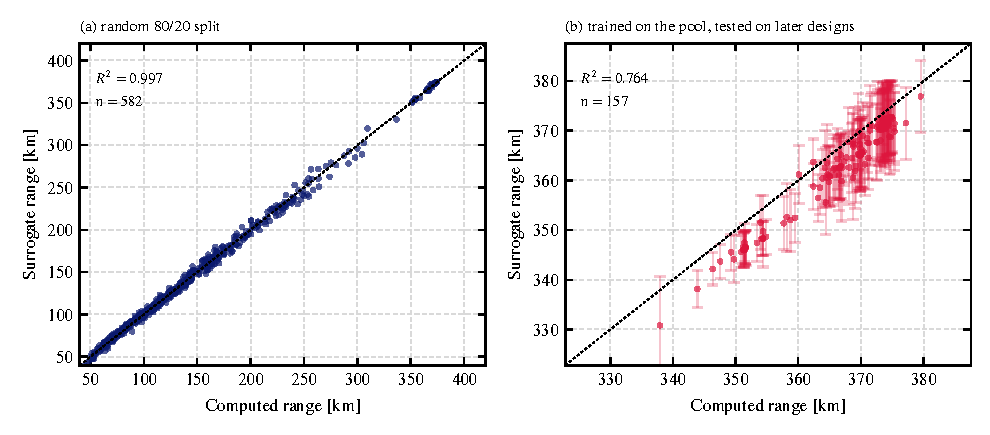
\includegraphics[width=\linewidth]{figures/fig_parity.pdf}
\caption{Surrogate model parity evaluation. (a) In-distribution random 80/20 split of the feasible designs of the database ($n=582$ test designs, $R^2 = 0.997$, $\mathrm{MAPE} = 2.3\%$). (b) Covariate distribution shift test: ensemble trained on the Latin hypercube pool and evaluated on the designs proposed by the original active-learning campaign ($n=157$, $R^2 = 0.764$, $\mathrm{MAE} = 3.7\,\mathrm{km}$, $\rho = 0.95$). Vertical error bars denote $\pm 1\bar{\sigma}$ epistemic uncertainty.}
\label{fig:surrogate_parity}
\end{figure}

\begin{table}[htbp]
\centering\small
\caption{Surrogate ensemble generalization and distribution shift audit metrics across aerodynamic targets.}
\label{tab:shift}
\resizebox{\linewidth}{!}{%
\begin{tabular}{@{}llrrrrrr@{}}
\toprule
Test & Target & $n_{\rm test}$ & $R^2$ & MAE & Bias & Spearman & 1-sd coverage \\
\midrule
train Phase1 $\to$ test Phase2 & range (km) & 157 & 0.76 & 3.72 & -3.68 & 0.95 & 0.78 \\
train range$<$250 $\to$ test range$\geq$250 & range (km) & 164 & 0.35 & 8.32 & -8.26 & 0.96 & 0.59 \\
train Phase1 $\to$ test Phase2 & $L/D$ & 157 & 0.89 & 0.11 & +0.03 & 0.94 & 0.97 \\
train range$<$250 $\to$ test range$\geq$250 & $L/D$ & 164 & 0.86 & 0.13 & -0.13 & 0.96 & 0.89 \\
train Phase1 $\to$ test Phase2 & static margin & 157 & 1.00 & 0.00 & +0.00 & 0.99 & 0.99 \\
train range$<$250 $\to$ test range$\geq$250 & static margin & 164 & 1.00 & 0.00 & -0.00 & 1.00 & 0.89 \\
\bottomrule
\end{tabular}

}
\end{table}

\section{Feasibility Boundary and Classifier Recall}
The constraints make $\NpoolInfeasShare\%$ of the pool infeasible, mainly through the static-margin band and the bay volume. The factorial runs of Section~\ref{sec:feas_ablation} show that the classifier is what keeps the global acquisition inside the feasible region at all, and the feasible fraction of the loop's evaluations (\NvValidALR\% for AL-R) remains below that of TuRBO (\NvValidTurbo\%), whose trust region achieves the same end geometrically.

The empirical audit in Section~\ref{sec:classifier_audit} and Table~\ref{tab:classifier_audit} explains the classifier recall characteristics. The global recall of $\NfnRecall\%$ is heavily influenced by class imbalance ($\NclfInfeasShare\%$ infeasible class) and boundary proximity: $\NfnWithin\%$ of misclassified valid designs lay within a $10\%$ margin of active constraint boundaries, compared to only $\NtpWithin\%$ for correctly accepted valid designs. While the median range among falsely rejected designs was $\NfnMedian\,\mathrm{km}$ (versus $\NtpMedian\,\mathrm{km}$ for correctly accepted designs), the largest range among falsely rejected designs averaged $\NfnMax\,\mathrm{km}$ over the splits, so the classifier boundary cuts close to the high-range region. In contrast, recall rises to \textbf{$\NfnTenRecall\%$} among the top 10\% of designs and \textbf{$\NfnTwoRecall\%$} among the top 2\% of high-range designs (evaluated on \NfnTwoN\ designs per test split). The classifier enters the acquisition function through a sigmoid weight $w(\mathcal{P}_{\mathrm{feas}})$ and not as a hard gate, so candidates with moderate feasibility confidence remain eligible for query whenever their predicted range or epistemic uncertainty is sufficiently large. Section~\ref{sec:feas_ablation} shows that a hard gate reaches the same range at the full budget but much later, which is consistent with this reading; probability-of-feasibility weighting has known limitations~\cite{cordelier2026multifidelity}.



\section{Benchmark: Intermediate Budgets, First Implementations and Interval Plot}
\label{sec:supp_benchmark}
Table~\ref{tab:anytime} repeats the benchmark comparison at intermediate budgets, Table~\ref{tab:asrun} lists the corrected baselines beside their first implementations, and Fig.~\ref{fig:forest} shows the headline differences of Table~\ref{tab:tests} with their intervals (filled squares are significant after Holm correction).

\begin{table}[htbp]
\centering\small
\caption{Mean running best feasible range (km, $\pm$ sd over seeds, pool included) at intermediate budgets, and differences between strategies with two-sided Welch $p$-values (not corrected for multiplicity).}
\label{tab:anytime}
\resizebox{\linewidth}{!}{%
\begin{tabular}{@{}lrrrrr@{}}
\toprule
Evaluations beyond the pool & 50 & 100 & 150 & 200 & 287 \\
\midrule
TuRBO ($n=20$) & 375.9 $\pm$ 6.6 & 382.9 $\pm$ 6.4 & 388.6 $\pm$ 5.9 & 393.3 $\pm$ 5.1 & 396.8 $\pm$ 4.4 \\
AL-R ($n=20$) & 370.3 $\pm$ 10.4 & 378.8 $\pm$ 7.6 & 383.8 $\pm$ 8.2 & 388.1 $\pm$ 6.0 & 391.5 $\pm$ 6.6 \\
AL ($n=11$) & 358.1 $\pm$ 7.3 & 374.1 $\pm$ 8.7 & 378.9 $\pm$ 8.4 & 382.7 $\pm$ 9.3 & 385.0 $\pm$ 10.4 \\
adapt10 ($n=20$) & 360.9 $\pm$ 8.3 & 372.9 $\pm$ 9.2 & 377.8 $\pm$ 7.1 & 381.9 $\pm$ 6.7 & 386.1 $\pm$ 6.3 \\
local10 ($n=10$) & 357.6 $\pm$ 4.7 & 358.8 $\pm$ 6.4 & 362.2 $\pm$ 4.9 & 363.4 $\pm$ 4.6 & 365.2 $\pm$ 4.7 \\
\midrule
TuRBO minus AL-R, km (Welch $p$) & +5.6 (0.051) & +4.1 (0.075) & +4.7 (0.043) & +5.2 (0.005) & +5.3 (0.005) \\
AL-R minus adapt10, km (Welch $p$) & +9.4 (0.003) & +5.9 (0.032) & +6.0 (0.017) & +6.2 (0.004) & +5.4 (0.011) \\
TuRBO minus adapt10, km (Welch $p$) & +15.0 ($<$0.001) & +10.0 ($<$0.001) & +10.8 ($<$0.001) & +11.3 ($<$0.001) & +10.7 ($<$0.001) \\
\bottomrule
\end{tabular}

}
\end{table}

\begin{table}[htbp]
\centering\small
\caption{Corrected baselines and their first implementations, which ranked new evaluations and pool designs on inconsistent energy bases; the last two rows are TuRBO with the sigmoid classifier weight in both versions. Columns as in Table~\ref{tab:budget}; ``(first)'' marks the implementation before the correction of the energy basis and ``+w'' the sigmoid classifier weight.}
\label{tab:asrun}
{\footnotesize\setlength{\tabcolsep}{4pt}\begin{tabular*}{\linewidth}{@{\extracolsep{\fill}}lrrrrrrrrr@{}}
\toprule
 & & \multicolumn{3}{c}{Best feasible range (km)} & \multicolumn{3}{c}{Share of evaluations (\%)} & \multicolumn{2}{c}{Beating the pool} \\
\cmidrule(lr){3-5}\cmidrule(lr){6-8}\cmidrule(l){9-10}
Strategy & Runs & at 100 & at 287 & min to max & valid & valid$_{60}$ & fail $g_8$ & runs & evals \\
\midrule
TuRBO & 20 & 382.9 & 396.8 $\pm$ 4.4 & 385.3 to 403.0 & 82 & 80 & 0 & 20/20 & 2 \\
TuRBO (first) & 10 & 381.0 & 396.6 $\pm$ 5.8 & 385.1 to 403.0 & 82 & 80 & 0 & 10/10 & 2 \\
adapt10 & 20 & 372.9 & 386.1 $\pm$ 6.3 & 369.2 to 393.2 & 68 & 69 & 0 & 20/20 & 34 \\
adapt10 (first) & 10 & 365.4 & 379.7 $\pm$ 4.5 & 370.8 to 386.4 & 71 & 72 & 0 & 10/10 & 51 \\
TuRBO+w & 10 & 383.9 & 397.5 $\pm$ 2.8 & 394.0 to 403.0 & 92 & 92 & 0 & 10/10 & 2 \\
TuRBO+w (first) & 10 & 376.8 & 394.8 $\pm$ 4.4 & 386.2 to 399.5 & 91 & 90 & 0 & 10/10 & 2 \\
\bottomrule
\end{tabular*}
}
\end{table}

\begin{figure}[htbp]
\centering
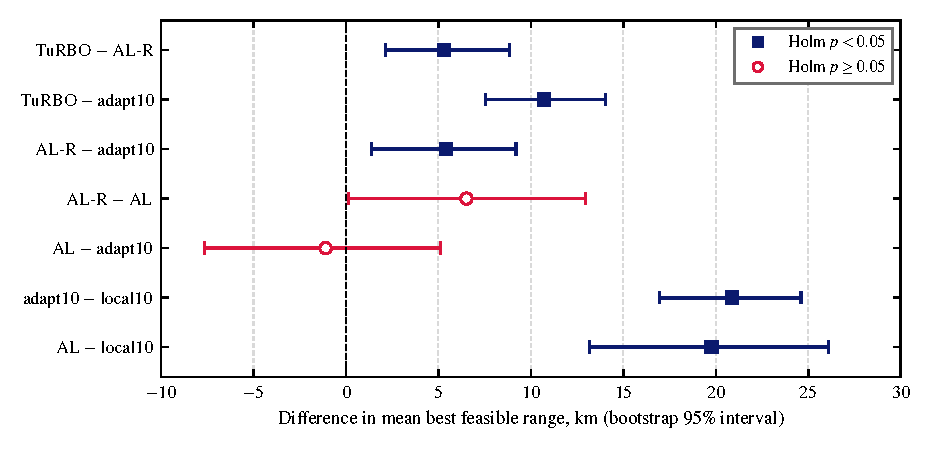
\includegraphics[width=0.88\linewidth]{figures/fig_forest.pdf}
\caption{Differences in mean best feasible range for the headline comparisons of Table~\ref{tab:tests}, with percentile bootstrap 95\% intervals. Filled squares are significant after Holm correction over the family; an interval that excludes zero can still fail the correction, as for AL-R against AL.}
\label{fig:forest}
\end{figure}


\section{Grid Convergence and Numerical Discretization Audit}
\label{sec:grid_convergence}
The sensitivity of the lattice solution to the panel density was examined on four designs that span the range of quality: the best design of active-learning replication 0, the pool best, the pool median and the pool 10th-percentile design. Mesh resolution was varied from $672$ panels ($1\times 12$ chordwise per section) to $3{,}584$ panels ($4\times 16$ chordwise per section), scaling panel density by a factor of 5.3.

\begin{table}[htbp]
\centering\small
\caption{Numerical grid convergence audit across 7 surface panel resolutions ($672$ to $3{,}584$ panels) for four representative configurations.}
\label{tab:grid}
\resizebox{\linewidth}{!}{%
\begin{tabular}{@{}lrrrrrr@{}}
\toprule
Design & Panels (span$\times$chord) & $C_L$ & $C_{D}$ & $L/D$ & $SM$ & Time (s) \\
\midrule
AL replication 0, best & 672 (1$\times$12) & 0.2561 & 0.01462 & 17.51 & 0.181 & 0.4 \\
AL replication 0, best & 1344 (2$\times$12) & 0.2561 & 0.01463 & 17.50 & 0.183 & 1.4 \\
AL replication 0, best & 1792 (2$\times$16) & 0.2561 & 0.01464 & 17.49 & 0.183 & 2.2 \\
AL replication 0, best & 2016 (3$\times$12) & 0.2561 & 0.01468 & 17.45 & 0.184 & 3.5 \\
AL replication 0, best & 2688 (2$\times$24) & 0.2561 & 0.01466 & 17.47 & 0.184 & 6.9 \\
AL replication 0, best & 2688 (3$\times$16) & 0.2561 & 0.01467 & 17.45 & 0.184 & 5.9 \\
AL replication 0, best & 3584 (4$\times$16) & 0.2561 & 0.01471 & 17.40 & 0.185 & 12.3 \\
Pool best & 672 (1$\times$12) & 0.2203 & 0.01400 & 15.74 & 0.193 & 0.5 \\
Pool best & 1344 (2$\times$12) & 0.2203 & 0.01397 & 15.77 & 0.195 & 1.6 \\
Pool best & 1792 (2$\times$16) & 0.2203 & 0.01399 & 15.74 & 0.196 & 2.2 \\
Pool best & 2016 (3$\times$12) & 0.2203 & 0.01400 & 15.73 & 0.196 & 3.2 \\
Pool best & 2688 (2$\times$24) & 0.2203 & 0.01403 & 15.70 & 0.196 & 5.6 \\
Pool best & 2688 (3$\times$16) & 0.2203 & 0.01402 & 15.71 & 0.196 & 5.3 \\
Pool best & 3584 (4$\times$16) & 0.2202 & 0.01417 & 15.54 & 0.194 & 10.7 \\
Pool median & 672 (1$\times$12) & 0.1143 & 0.01482 & 7.71 & 0.102 & 0.4 \\
Pool median & 1344 (2$\times$12) & 0.1142 & 0.01482 & 7.71 & 0.104 & 1.8 \\
Pool median & 1792 (2$\times$16) & 0.1143 & 0.01495 & 7.64 & 0.104 & 2.4 \\
Pool median & 2016 (3$\times$12) & 0.1142 & 0.01596 & 7.16 & 0.107 & 3.0 \\
Pool median & 2688 (2$\times$24) & 0.1143 & 0.01508 & 7.58 & 0.104 & 5.4 \\
Pool median & 2688 (3$\times$16) & 0.1142 & 0.01505 & 7.59 & 0.104 & 5.2 \\
Pool median & 3584 (4$\times$16) & 0.1146 & 0.01656 & 6.92 & 0.104 & 12.4 \\
Pool 10th percentile & 672 (1$\times$12) & 0.0694 & 0.01335 & 5.20 & 0.144 & 0.4 \\
Pool 10th percentile & 1344 (2$\times$12) & 0.0693 & 0.01333 & 5.20 & 0.146 & 1.6 \\
Pool 10th percentile & 1792 (2$\times$16) & 0.0693 & 0.01348 & 5.15 & 0.146 & 2.5 \\
Pool 10th percentile & 2016 (3$\times$12) & 0.0693 & 0.01337 & 5.18 & 0.146 & 3.1 \\
Pool 10th percentile & 2688 (2$\times$24) & 0.0693 & 0.01363 & 5.09 & 0.146 & 6.1 \\
Pool 10th percentile & 2688 (3$\times$16) & 0.0693 & 0.01351 & 5.13 & 0.146 & 5.4 \\
Pool 10th percentile & 3584 (4$\times$16) & 0.0776 & 0.01876 & 4.14 & 0.136 & 13.7 \\
\bottomrule
\end{tabular}

}
\end{table}

Table~\ref{tab:grid} shows the following.
\begin{itemize}
    \item For the two good designs the production grid is adequate. For the best design of active-learning replication 0 the lift coefficient is unchanged to four digits and $L/D$ deviates by at most $0.55\%$ from the 1{,}344-panel value ($0.62\%$ between the coarsest and the finest grid, $17.51$ versus $17.40$). For the pool best, $L/D$ changes by at most $1.45\%$.
    \item $L/D$ decreases slowly with spanwise refinement on every design, so the sequence is not asymptotically converged and no extrapolated value is quoted.
    \item For the two poor designs the finest grid departs strongly from the others ($L/D$ lower by $10.3\%$ for the pool median and $20.5\%$ for the 10th-percentile design, with a jump in $C_L$ for the latter). These designs have closely spaced sections, for which a fine spanwise panelling makes the influence matrix poorly conditioned; this is the reason the production grid uses two spanwise panels per interval. The ordering of the four designs is the same on every grid.
    \item The static margin changes by less than $\NgridSM$ across all grids and designs, and by $0.004$ for the best design.
    \item One evaluation takes $0.4\,\mathrm{s}$ at 672 panels, $1.4\,\mathrm{s}$ at 1{,}344 and $12.3\,\mathrm{s}$ at 3{,}584.
\end{itemize}



\section{Viscous Section Drag Verification with NeuralFoil}
\label{sec:neuralfoil_audit}
The strip estimate of profile drag was compared with NeuralFoil section polars under free transition and with forced transition near the leading edge, for the five designs of the Euler study.

\begin{table}[htbp]
\centering\small
\caption{Viscous profile drag comparison between Raymer empirical strip theory and NeuralFoil ($e^N$ free transition vs.\ fully turbulent) across five configurations.}
\label{tab:visc}
\resizebox{\linewidth}{!}{%
\begin{tabular}{@{}lrrrr@{}}
\toprule
Design & Raymer, $x_{tr}=0.40$ & NeuralFoil, free transition & NeuralFoil, fully turbulent & Ratio NF/Raymer \\
\midrule
Original campaign, best & 102 & 66 & 120 & 0.64 \\
AL replication 0, best & 103 & 67 & 121 & 0.65 \\
Pool best & 100 & 63 & 118 & 0.63 \\
Pool median & 92 & 55 & 108 & 0.60 \\
Pool 10th percentile & 87 & 54 & 104 & 0.62 \\
\bottomrule
\end{tabular}

}
\end{table}

With free transition and at the cruise lift coefficient, NeuralFoil gives $0.60$ to $0.65$ times the strip estimate (Table~\ref{tab:visc}, Fig.~\ref{fig:fidelity_suite}b), and $\NnfLo$ to $\NnfHi$ times when the section lift coefficient is varied by $\pm 0.1$; with forced transition it gives about $1.18$ times. The strip estimate with its fixed transition at $40\%$ chord thus lies between the two, closer to the turbulent value. The ratio varies little between designs, so the profile-drag ranking of these five designs is the same under both models. The absolute level is another matter: for the best design of the original campaign, replacing the strip estimate by the free-transition value would lower total drag by about a quarter and raise $L/D$ and range by about a third. Absolute range therefore depends strongly on how much laminar flow the built airframe achieves, which this study cannot determine.



\section{Euler CFD Comparison of Lift and Static Margin}
\label{sec:cfd_validation}
Three-dimensional effects were checked with inviscid compressible Euler solutions (SU2) of five designs: the best design of active-learning replication 0, the pool best, the pool median, the pool 10th-percentile design and the best design of the original campaign. The half model includes the wing and winglet without the nacelle. Unstructured tetrahedral volume meshes of approximately $1.2 \times 10^5$ nodes ($118{,}711$ to $126{,}806$ nodes, surface mesh sizing $h = 7\,\mathrm{mm}$) were generated using Gmsh, and steady solutions were computed at the cruise Mach number ($M \approx 0.11$) at the lattice cruise angle of attack and $2^\circ$ above it. Euler drag is not used: at this resolution it is dominated by numerical dissipation.

\begin{table}[htbp]
\centering\small
\caption{Comparison of three-dimensional compressible Euler solutions (SU2) with the lattice predictions for five representative designs.}
\label{tab:cfd}
\resizebox{\linewidth}{!}{%
\begin{tabular}{@{}lrrrrrr@{}}
\toprule
Design & $C_L$ Euler & $C_L$ VLM & $C_L$ ratio & $SM$ Euler & $SM$ VLM & $SM$ ratio \\
\midrule
AL replication 0, best & 0.2478 & 0.2561 & 0.97 & 0.221 & 0.183 & 1.21 \\
Pool best & 0.2168 & 0.2203 & 0.98 & 0.228 & 0.195 & 1.17 \\
Pool median & 0.1216 & 0.1142 & 1.06 & 0.132 & 0.104 & 1.28 \\
Pool 10th percentile & 0.0827 & 0.0693 & 1.19 & 0.175 & 0.146 & 1.20 \\
Original campaign, best & 0.2559 & 0.2471 & 1.04 & 0.258 & 0.225 & 1.14 \\
\bottomrule
\end{tabular}

}
\end{table}

As documented in Table~\ref{tab:cfd} and Fig.~\ref{fig:fidelity_suite}(c):
\begin{itemize}
    \item \textbf{Lift.} The ratio $C_{L,\mathrm{Euler}} / C_{L,\mathrm{VLM}}$ lies between $0.97$ and $1.04$ for the three designs with a cruise $C_L$ above $0.2$ and rises to $1.06$ and $1.19$ for the two low-lift designs. The Euler mesh is itself not converged to this level: on the best design of replication 0, refining the surface size from $10$ to $7\,\mathrm{mm}$ changes $C_L$ from $0.262$ to $0.248$ ($5.5\%$). The agreement in lift is therefore within the discretization uncertainty of the Euler solution and is not a validation to a few percent.
    \item \textbf{Static margin.} The Euler static margin is higher than the lattice value on all five designs, by a factor of $1.14$ to $1.28$ (\NcfdChampSM\ versus \NchSM\ for the best design of the original campaign). A lattice on the camber surface carries no thickness, and the thick center body is a plausible source of the difference, but the mechanism was not isolated. The consequence matters for the constraint: because the lattice underpredicts the margin, it is not conservative with respect to the upper limit $SM \le 0.25$. The best design of the original campaign has $SM = 0.258$ in the Euler solution and violates the limit, whereas the best design of replication 0 has $SM = 0.221$ (lattice $0.183$). Section~\ref{sec:sm_calibration} extends the comparison to \NcalN\ designs and shows that the difference is an almost constant additive offset.
\end{itemize}


\begin{figure}[htbp]
\centering
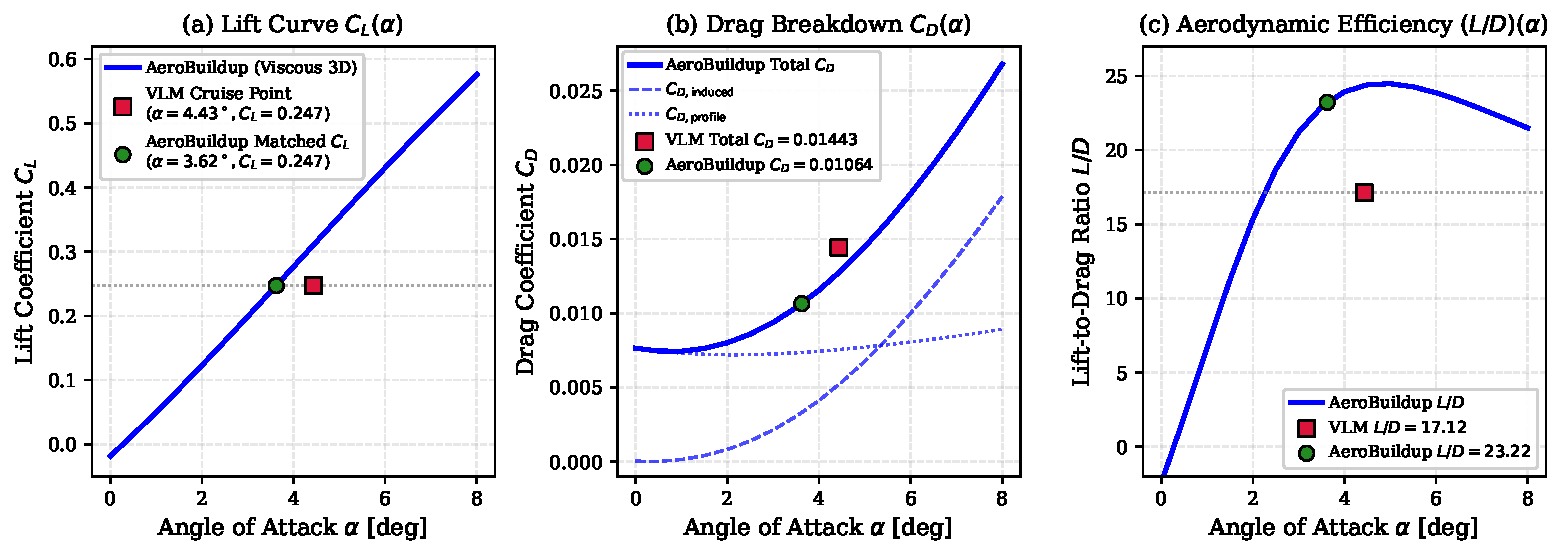
\includegraphics[width=\linewidth]{figures/figure8_vlm_vs_aerobuildup.pdf}
\caption{Aerodynamic sweep comparing the baseline potential-flow VLM pipeline against viscous-corrected AeroBuildup for the original-campaign champion configuration across angle of attack $\alpha \in [0^\circ, 8^\circ]$. (a) Lift curve $C_L(\alpha)$ with matched cruise operating point ($C_{L,\mathrm{cruise}} = 0.247$, crimson square: VLM at $\alpha = 4.43^\circ$; green circle: AeroBuildup at $\alpha = 3.62^\circ$). (b) Drag coefficient breakdown $C_D(\alpha)$ into total drag, induced drag ($C_{D,\mathrm{induced}}$, dashed), and profile drag ($C_{D,\mathrm{profile}}$, dotted). (c) Aerodynamic efficiency $(L/D)(\alpha)$ versus angle of attack, showing cruise efficiency of $L/D = 23.22$ at matched cruise lift (versus VLM $17.12$) and peak efficiency reaching $\approx 24.5$ near $\alpha \approx 5^\circ$.}
\label{fig:aerobuildup_polar}
\end{figure}


\section{Re-Ranking Under the Calibrated Constraint and Audited Designs}
\label{sec:supp_rerank}
Table~\ref{tab:sm_rerank} belongs to Section~\ref{sec:sm_calibration} of the main text and Table~\ref{tab:best} to Section~\ref{sec:champion_characteristics}.

\begin{table}[htbp]
\centering\small
\caption{Best-of-run range with the original lattice margin constraint and after applying the CFD calibration of the margin, by search strategy (corrected implementations). The last column counts runs whose best design lies outside the calibrated band $0.05 \le SM \le 0.25$.}
\label{tab:sm_rerank}
\resizebox{\linewidth}{!}{%
\begin{tabular}{@{}lrrrrr@{}}
\toprule
Search & Runs & Best, VLM margin (km) & Best, calibrated margin (km) & Mean loss (km) & Runs whose best design leaves the band \\
\midrule
AL, sigmoid weight & 10 & 385.5 & 385.5 & 0.0 & 0 of 10 \\
AL-R & 20 & 391.5 & 391.2 & 0.2 & 4 of 20 \\
TuRBO & 20 & 396.8 & 396.7 & 0.0 & 1 of 20 \\
TuRBO, with sigmoid weight & 10 & 397.5 & 397.5 & 0.0 & 0 of 10 \\
AL, hard 0/1 gate & 10 & 394.0 & 393.1 & 0.9 & 3 of 10 \\
Adaptive local, 10\% & 20 & 386.1 & 385.9 & 0.2 & 3 of 20 \\
Local, 10\% & 10 & 365.2 & 362.1 & 3.1 & 4 of 10 \\
Local, 5\% & 10 & 364.2 & 363.9 & 0.3 & 1 of 10 \\
Fresh LHS & 10 & 298.3 & 291.0 & 7.3 & 2 of 10 \\
Uniform random & 10 & 307.6 & 306.0 & 1.6 & 2 of 10 \\
\bottomrule
\end{tabular}

}
\end{table}

\begin{table}[htbp]
\centering\small
\caption{Characteristics of the best design of the original campaign and of the best design of active-learning replication 0.}
\label{tab:best}
\begin{tabular}{@{}lrr@{}}
\toprule
 & Original campaign & AL replication 0, best \\
\midrule
Range, as optimized (km) & 379.6 & 394.4 \\
Range with battery mass set to 3.400\,kg (km) & 379.4 & 385.2 \\
Battery mass variable (kg) & 3.402 & 3.499 \\
$L/D$ & 17.12 & 17.50 \\
$C_L$ & 0.247 & 0.256 \\
$S_\mathrm{ref}$ (m$^2$), aspect ratio & 0.402, 5.59 & 0.396, 5.68 \\
All-up mass (kg) & 7.96 & 8.04 \\
Cruise speed (km/h) & 132 & 131 \\
$SM$, lattice & 0.225 & 0.183 \\
$SM$, Euler CFD & 0.258 & 0.221 \\
$C_m$ at cruise & -0.019 & -0.013 \\
Trim drag (\% of $C_D$) & 1.1 & 0.5 \\
\bottomrule
\end{tabular}

\end{table}


\section{Battery Pack and Energy Basis}
\label{sec:battery_pack}
Energy storage is formulated around the cylindrical Samsung INR21700-50E lithium-ion cell, possessing manufacturer specifications of 5.0\,Ah capacity, 3.6\,V nominal voltage, and 69\,g mass ($18.0$\,Wh per cell, corresponding to $260.9\,\mathrm{Wh/kg}$ at the cell level). 

A 6-series, 8-parallel (6S8P) topology comprising 48 cells ($21.6\,\mathrm{V}$ nominal, $40.0\,\mathrm{Ah}$) yields a nominal storage capacity of \NpackNom\,Wh. The physical mass of the 48 cells is $48 \times 0.069\,\mathrm{kg} = 3.312\,\mathrm{kg}$. Accounting for $0.088\,\mathrm{kg}$ of nickel busbar interconnects, insulation wrap, Battery Management System (BMS) wiring, and structural end-caps, the complete pack mass is taken as $3.400\,\mathrm{kg}$, which is close to the battery mass of the best design of the original campaign ($m_{\mathrm{b}} = \Nchmbat\,\mathrm{kg}$). This configuration delivers a pack-level nominal energy density of $254.1\,\mathrm{Wh/kg}$. Enforcing an 80\% maximum depth-of-discharge (DoD) reserve to account for climb, loiter reserves, headwind margins, and cyclic degradation, the usable pack energy density is:
\begin{equation}
e_u = 0.80 \times 254.1\,\mathrm{Wh/kg} = \NeU\,\mathrm{Wh/kg} = \NeUkJ\,\mathrm{kJ/kg}
\end{equation}

The underlying 10,087-run optimization dataset was initially evaluated using a conservative baseline specification of $e_{u,\mathrm{base}} = 160.0\,\mathrm{Wh/kg}$ ($576.0\,\mathrm{kJ/kg}$). Because Eq.~\eqref{eq:breguet_range} is strictly linear in usable energy density $e_u$ for any fixed design vector $\mathbf{x}$, and because $e_u$ does not enter into any aerodynamic, volumetric, or stability feasibility condition in $\mathcal{F}(\mathbf{x})$, all range outputs from the computational database scale by the exact constant factor:
\begin{equation}
f_{\mathrm{energy}} = \frac{e_u}{e_{u,\mathrm{base}}} = \frac{\NeU\,\mathrm{Wh/kg}}{160.0\,\mathrm{Wh/kg}} = \NeF
\end{equation}
This scaling preserves the ordering of all evaluated designs and every statistical comparison, and it ties the reported ranges to a 48-cell 21700 pack that can be built. The battery mass remains a continuous design variable in the search; designs at the $3.5\,\mathrm{kg}$ bound therefore carry slightly more than this pack, and Table~\ref{tab:best} also reports the range with the battery mass set to $3.400\,\mathrm{kg}$. At cruise velocity, the discharge current is approximately 1.4\,A per cell ($0.28$\,C), well below the continuous discharge rating of 9.8\,A.



\section{Solver Settings of the Verification Tools}
\label{sec:mf_architecture}
Three tools are used to check the low-order pipeline; none of them is used inside the optimization. They are not fully independent of each other: AeroBuildup takes its section polars from NeuralFoil.
\begin{enumerate}
    \item \textbf{AeroBuildup Viscous Strip Theory:} Implemented in AeroSandbox, AeroBuildup couples low-aspect-ratio lifting line calculations with embedded 2D section polar databases, applying empirical corrections for sweep, taper, and viscous boundary-layer growth.
    \item \textbf{NeuralFoil Deep Neural Polar Engine:} Developed by Sharpe~\cite{sharpe2024neuralfoil}, NeuralFoil is a neural surrogate trained on XFoil viscous boundary-layer solutions across $Re \in [10^4, 10^7]$ and Mach $\le 0.4$. It predicts section $c_l$, $c_d$ and $c_m$, including the effect of natural transition as XFoil's $e^N$ method predicts it, so no transition location has to be assumed.
    \item \textbf{SU2 3D Compressible Euler CFD:} For compressible 3D verification, the open-source finite-volume solver SU2~\cite{economon2016su2} is executed on unstructured tetrahedral volume grids generated with Gmsh~\cite{geuzaine2009gmsh}. Calculations solve the 3D compressible Euler equations:
    \begin{equation}
    \frac{\partial \mathbf{U}}{\partial t} + \nabla \cdot \mathbf{F}(\mathbf{U}) = 0
    \end{equation}
    using Roe flux difference splitting with second-order MUSCL reconstruction~\cite{roe1981approximate}, the Venkatakrishnan slope limiter~\cite{venkatakrishnan1993limiter}, and implicit time stepping with an adaptive CFL number. The Euler meshes employ approximately $1.2 \times 10^5$ nodes ($118{,}711$ to $126{,}806$ nodes) with surface mesh sizing of $h = 7\,\mathrm{mm}$ to capture leading-edge expansions and spanwise pressure distributions.
\end{enumerate}



